\chapter{Implementasi Program dan Pengujian}

Pada bab ini, akan dijelaskan tentang lingkupan pembangunan, implementasi rancangan antarmuka, serta pengujian secara fungsional dan experimental pada aplikasi \textsl{data mining}.

\section{Lingkungan Pembangunan}
Lingkungan perangkat lunak dan perangkat keras yang digunakan untuk membangun aplikasi \textsl{data mining} ini:

\begin{enumerate}
	\item CPU
	\begin{itemize}
		\item Prosesor: Intel(R) Core(TM) i7, 1.60 GHz
		\item Memori ram: 6 GB
		\item VGA: NVDIA GeForce GT 330M
		\item Hardisk: 300 GB
	\end{itemize}
	\item Sistem operasi: Windows 7 Professional
	\item Platform: NetBeans IDE 8.0
\end{enumerate}

\section{Implementasi Rancangan Antarmuka}
Pada aplikasi \textsl{data mining} ini, terdapat dua form. Form pertama berfungsi untuk memilih file CSV yang akan dilakukan \textsl{data mining}, memilih metode pembuatan \textsl{decision tree}, serta menunjukkan hasil \textsl{decision tree} yang dihasilkan dalam bentuk String. Sedangkan untuk form kedua, berfungsi untuk memvisualisasikan \textsl{decision tree} yang sudah diperoleh dalam bentuk gambar.

TextField yang pertama berfungsi untuk mengisi alamat file CSV yang akan dilakukan \textsl{data mining}. RadioButton berfungsi untuk memilih metode manakah yang akan digunakan untuk membuat \textsl{decision tree}, sedangkan TextArea digunakan untuk memperlihatkan hasil \textsl{decision tree} dalam bentuk String.

\begin{figure}[H]
\centering
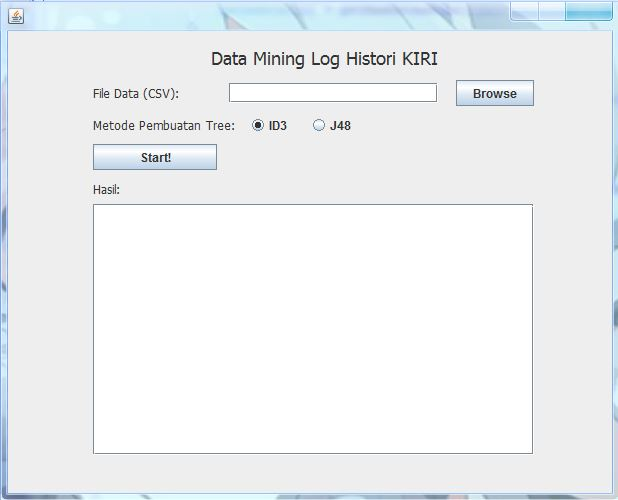
\includegraphics[scale=0.7]{Gambar/GUI1.jpg}
\caption[Tampilan Form Awal Aplikasi \textsl{Data Mining}]{Tampilan Form Awal Aplikasi \textsl{Data Mining}} 
\label{fig:GUI1}
\end{figure}

Terdapat dua cara untuk mengisi TextField, yaitu ditulis secara manual alamat file CSV atau dengan cara mengklik tombol button browse dan memilih file CSV pada FileSelector.

\begin{figure}[H]
\centering
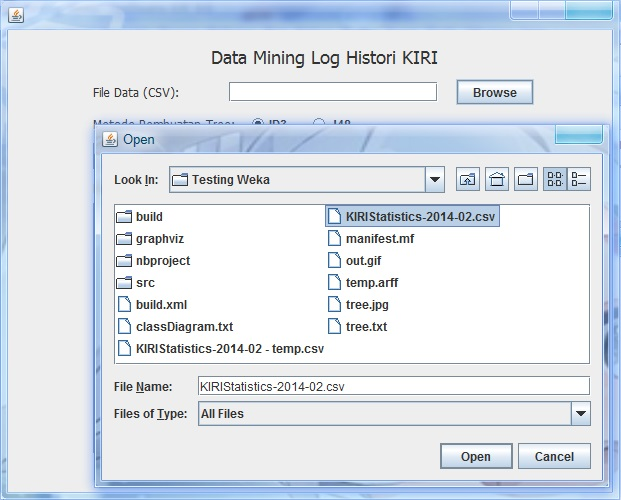
\includegraphics[scale=0.7]{Gambar/GUI2.jpg}
\caption[Tampilan FileSelector untuk Memilih File CSV]{Tampilan FileSelector untuk Memilih File CSV} 
\label{fig:GUI2}
\end{figure}

\begin{figure}[H]
\centering
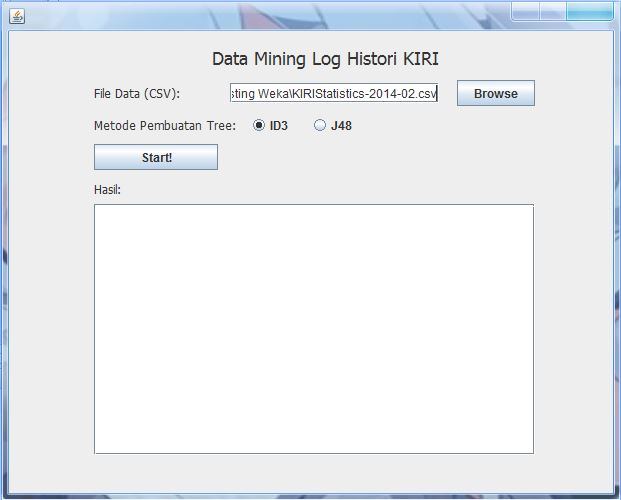
\includegraphics[scale=0.7]{Gambar/GUI3.jpg}
\caption[Tampilan Form setelah Memilih File CSV]{Tampilan Form setelah Memilih File CSV} 
\label{fig:GUI3}
\end{figure}

Setelah alamat file CSV diisi, hal selanjutnya yang dilakukan adalah memilih metode pembuatan \textsl{decision tree} pada RadioButton. RadioButton akan memilih metode ID3 jika \textsl{setting} ini tidak diubah.

\begin{figure}[H]
\centering
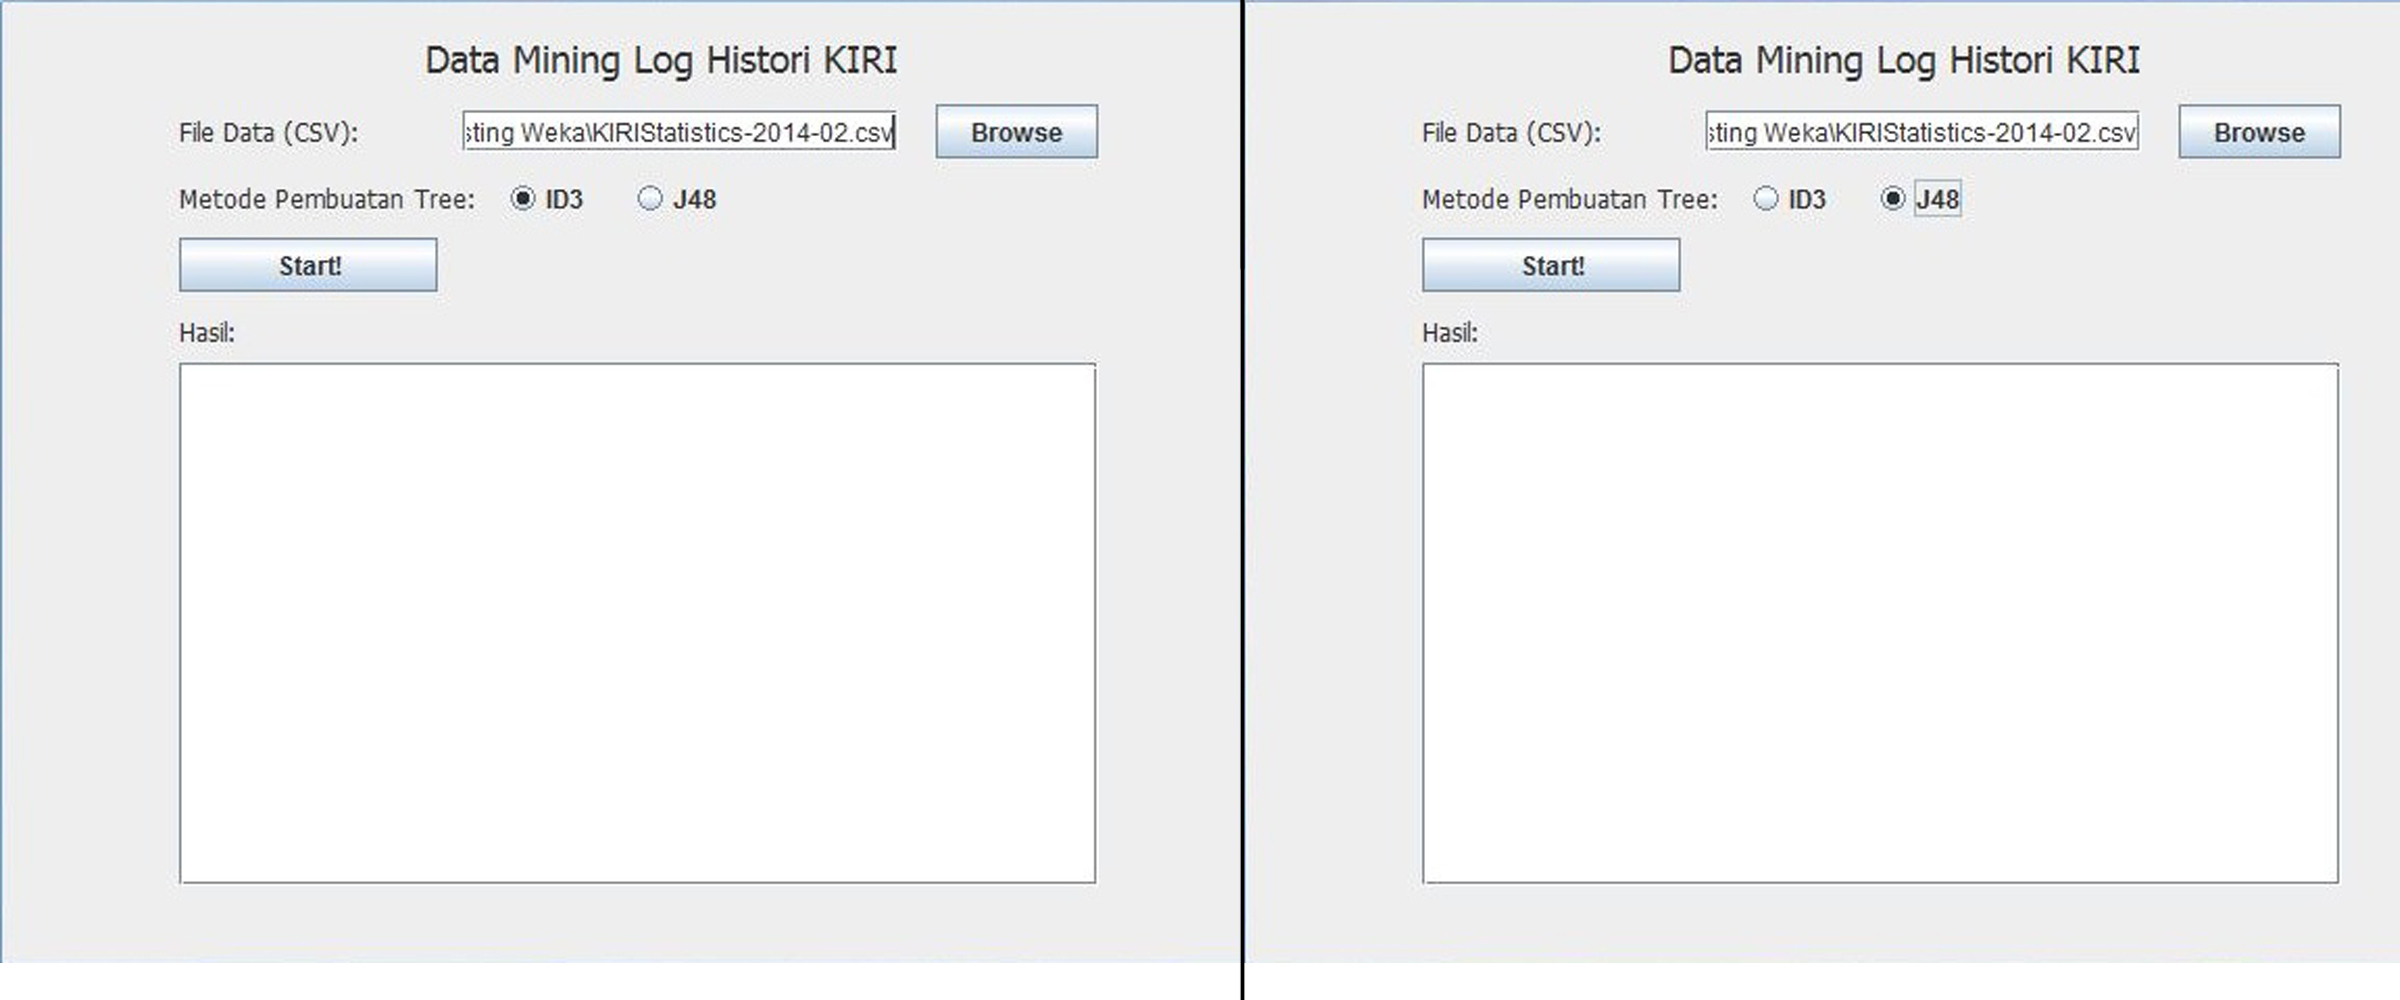
\includegraphics[scale=0.7]{Gambar/GUI3and4.jpg}
\caption[Tampilan Form Pemilihan Metode Pembuatan \textsl{Decision Tree}]{Tampilan Form Pemilihan Metode Pembuatan \textsl{Decision Tree}} 
\label{fig:GUI3and4}
\end{figure}

Kemudian, tombol start diklik lalu program akan melakukan proses \textsl{data mining}. Setelah selesai, maka program akan menunjukkan hasil \textsl{data mining} dalam bentuk String pada TextArea dan dalam bentuk gambar pada form kedua.

\begin{figure}[H]
\centering
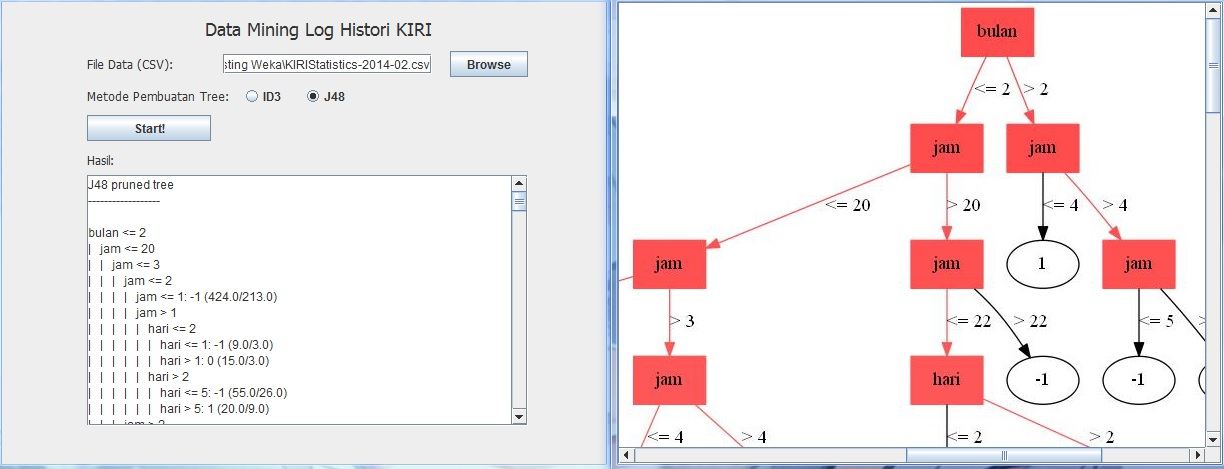
\includegraphics[scale=0.5]{Gambar/GUI5.jpg}
\caption[Tampilan Form Menampilkan Hasil \textsl{Data Mining}]{Tampilan Form Menampilkan Hasil \textsl{Data Mining}} 
\label{fig:GUI5}
\end{figure}

\section{Pengujian Aplikasi \textsl{Data Mining}}

\subsection{Rancangan Pengujian}

Dalam pengujian aplikasi \textsl{data mining} ini, akan digunakan teknik pengujian \textsl{black box}. Pengujian yang akan dilakukan:
\begin{enumerate}
	\item Pengujian \textsl{method} utama untuk mencapai tujuan dari aplikasi \textsl{data mining} ini. Terdapat beberapa \textsl{method} yang perlu diuji, yaitu
	\begin{enumerate}
		\item \textsl{method} untuk membaca file CSV
		\item \textsl{method} untuk melakukan \textsl{preprocessing data}
		\item \textsl{method} untuk membuat \textsl{decision tree}
		\item \textsl{method} untuk mengubah \textsl{decision tree} dalam bentuk String menjadi bahasa DOT
	\end{enumerate}
	\item Kebenaran perangkat lunak hanya dilihat pada hasil keluaran program atau kondisi masukan yang diberikan tanpa melihat bagaimana proses untuk mendapatkan keluaran tersebut.
	\item Dari keluaran yang dihasilkan, kemampuan program untuk memenuhi kebutuhan pemakai dapat diukur dan dapat diketahui kesalahan jika ada.
\end{enumerate}


























